\section{Design Language}

The design language or sometimes called design vocabulary is the design guide lines for \projectname{}. Each object there is important in the application have gotten their own unique feel.

\subsection{Color scheme}

\begin{figure}[htb]
    \centering
    
\includegraphics[width=\textwidth]{gfx/color_schema.pdf}
    \caption{color schema of \projectname{}.}
    \label{fig:color_schema}
\end{figure}

The color schema seen in \figref{fig:color_schema} shows the colors which is used in the applications design.

\subsection{Fonts}

The family of fonts will be: Arial, Helvetica. These fonts have been selected because they are common both in Windows and Mac and therefore can be called browser safe \cite{common_fonts}.

\subsection{Shapes}

All boxes which is possible to interact with in the application have rounded corners. This was done because the interaction for the user should be simple and straight forward.

\subsection{Layouts}

\begin{figure}[htb]
    \centering
    
\includegraphics[width=\textwidth]{gfx/menu.pdf}
    \caption{The menu of the application, with the control menu point activated.}
    \label{fig:menu_design}
\end{figure}

In \figref{fig:menu_design} the menu of the application is seen. The control menu point is active and therefore is represented with a gray color. Else the menu is black and with white spacers.

\begin{figure}[htb]
    \centering
    
\includegraphics[width=\textwidth]{gfx/search.pdf}
    \caption{Search bar of the application}
    \label{fig:search_bar_design}
\end{figure}

In \figref{fig:search_bar_design} the search bar of the application is seen. The ``search'' text will disappear when clicked and if the user types anything this will be shown in the search bar instead.

\begin{figure}[htb]
    \centering
    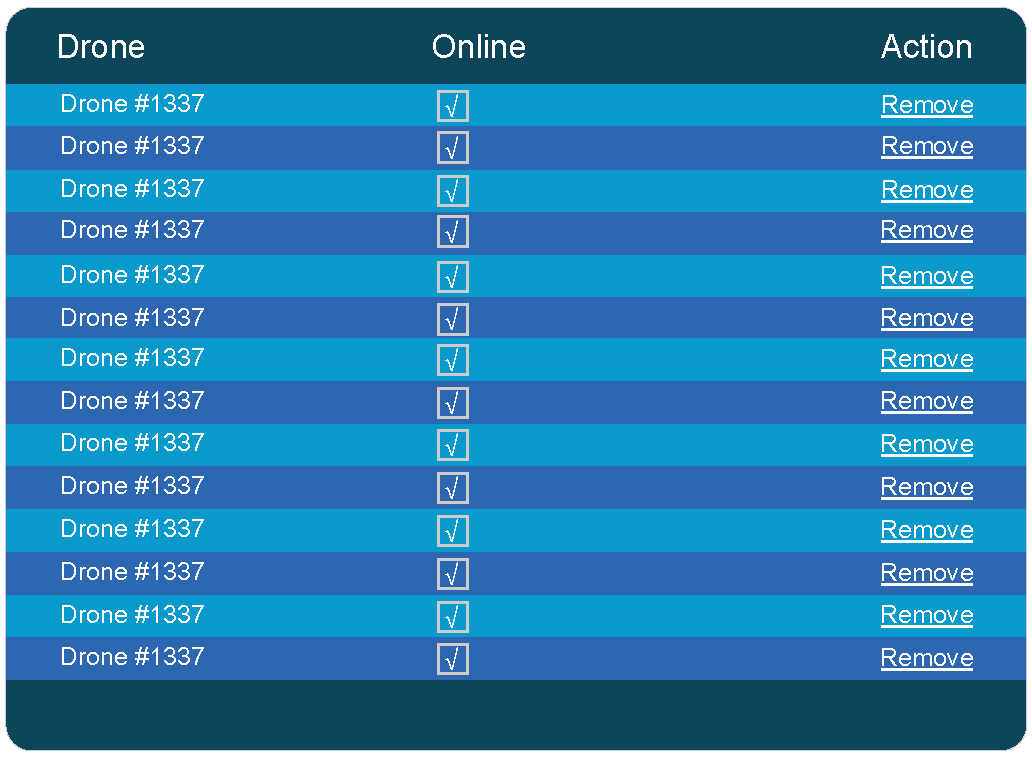
\includegraphics[width=\textwidth]{gfx/table.pdf}
    \caption{Table design for the application.}
    \label{fig:table_design}
\end{figure}

In \figref{fig:table_design} the general design for tables of the application is seen. 

\begin{figure}[htb]
    \centering
    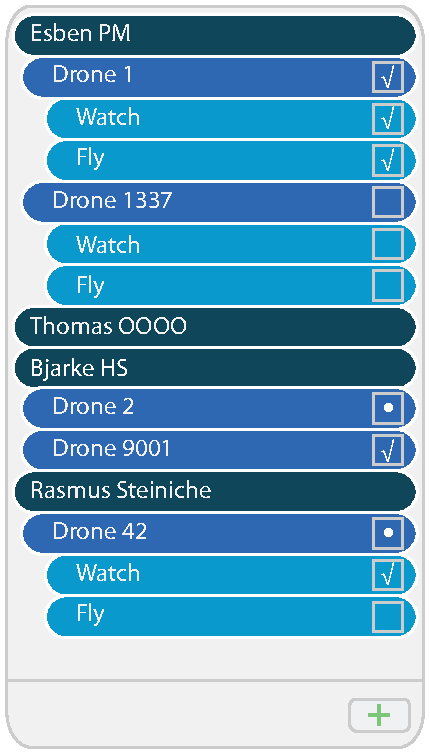
\includegraphics[scale=1.0]{gfx/list.pdf}
    \caption{List design for the application.}
    \label{fig:list_design}
\end{figure}

\begin{figure}[htb]
    \centering
    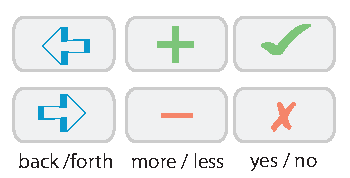
\includegraphics[scale=1.0]{gfx/button.pdf}
    \caption{Button design for the application.}
    \label{fig:button_design}
\end{figure}